%% ------------------------------------------------------------------------- %%
\chapter{Introdução}
\label{cap:introducao}

%% ------------------------------------------------------------------------- %%
\section{Considerações Preliminares}
\label{sec:consideracoes_preliminares}

Projetos de Software Livre (SL) típicos normalmente recebem a
colaboração de pessoas geograficamente distantes \cite{Dempsey1999} e
se organizam ao redor de um ou mais líderes.

Num primeiro momento, este fato poderia indicar que esse tipo de
projeto não é candidato para o uso de métodos ágeis de desenvolvimento
de software já que alguns valores essenciais parecem ausentes. Por
exemplo, a distância entre os desenvolvedores e a diversidade entre
suas culturas dificulta muito a comunicação, que é um dos principais
valores de métodos ágeis. No entanto, a maioria dos projetos de
software livre compartilham alguns princípios e mesmo valores
enunciados no manifesto ágil \cite{AgileManifesto}. Adaptação a
mudanças, trabalhar com \emph{feedback} contínuo, entregar
funcionalidades reais, respeitar colaboradores e usuários e enfrentar
desafios são atitudes esperadas de desenvolvedores de métodos ágeis
que são naturalmente encontradas em comunidades de Software Gratuito,
Livre e Aberto (FLOSS - \emph{Free, Libre and Open Source Software}).

Durante um \emph{workshop} \cite{OOPSLA07} sobre \emph{``No Silver
  Bullets''} \cite{Brooks1987} na conferência OOPSLA 2007, métodos
ágeis e software livre foram mencionados
\footnote{\url{http://mysite.verizon.net/dennis.mancl/oopsla07/silver_report.html\#issue4}
  - Último acesso 26/09/2009} como ``duas balas de prata fracassadas''
que trouxeram grandes benefícios à comunidade de software apesar de
não terem resolvido de forma completa os problemas ligados ao
desenvolvimento de software. Durante o mesmo \emph{workshop},
perguntou-se se o uso de várias ``balas de prata fracassadas'' não
poderia fazer o papel de uma bala de prata real, isto é, aumentar em
uma ordem de magnitude os níveis de produção de software.

Em uma conferência que ocorreu em São Paulo no dia 11 de Outubro de
2008 e reuniu aproximadamente 200 pessoas interessadas em métodos
ágeis\footnote{Encontro Ágil - \url{http://encontroagil.com.br/} -
  Último acesso: 01/06/2009}, o autor desse trabalho realizou uma
pesquisa para descobrir se a associação entre métodos ágeis e software
livre é comum. Uma pesquisa (disponível no Apêndice \ref{ape:EA}) foi
realizada em papel e entregue a todos os participantes do encontro no
início do evento e recolhida ao final do evento. Foram coletados 93
formulários preenchidos que resultaram nas seguintes estatísticas.

% TODO Aumentar legendas

\begin{figure}[htb]
  \begin{minipage}[t]{0.5\linewidth}
    \centering
    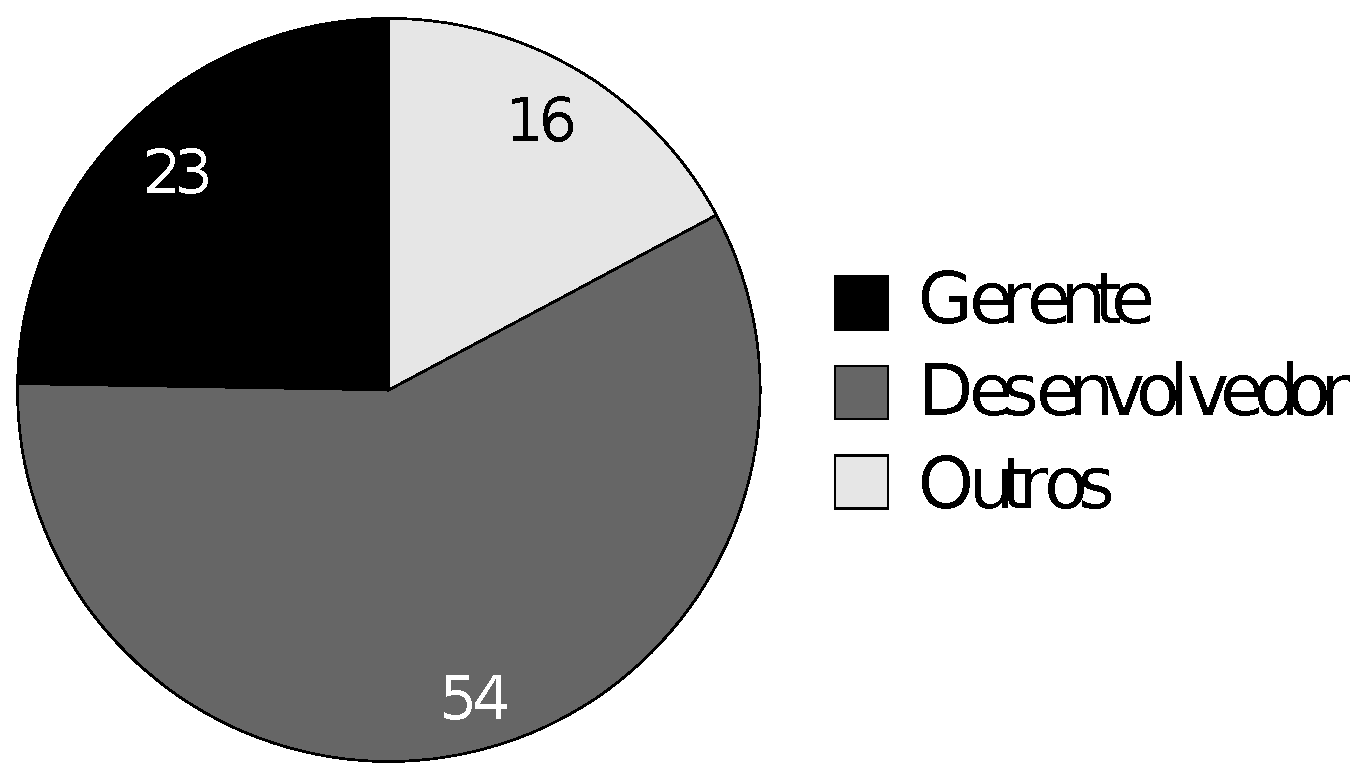
\includegraphics[scale=.3]{EA-atividades}
    \caption{Atividades desempenhadas pelos participantes da pesquisa}
    \label{fig:EA-atividades}
  \end{minipage}
  \begin{minipage}[t]{0.5\linewidth}
    \centering
    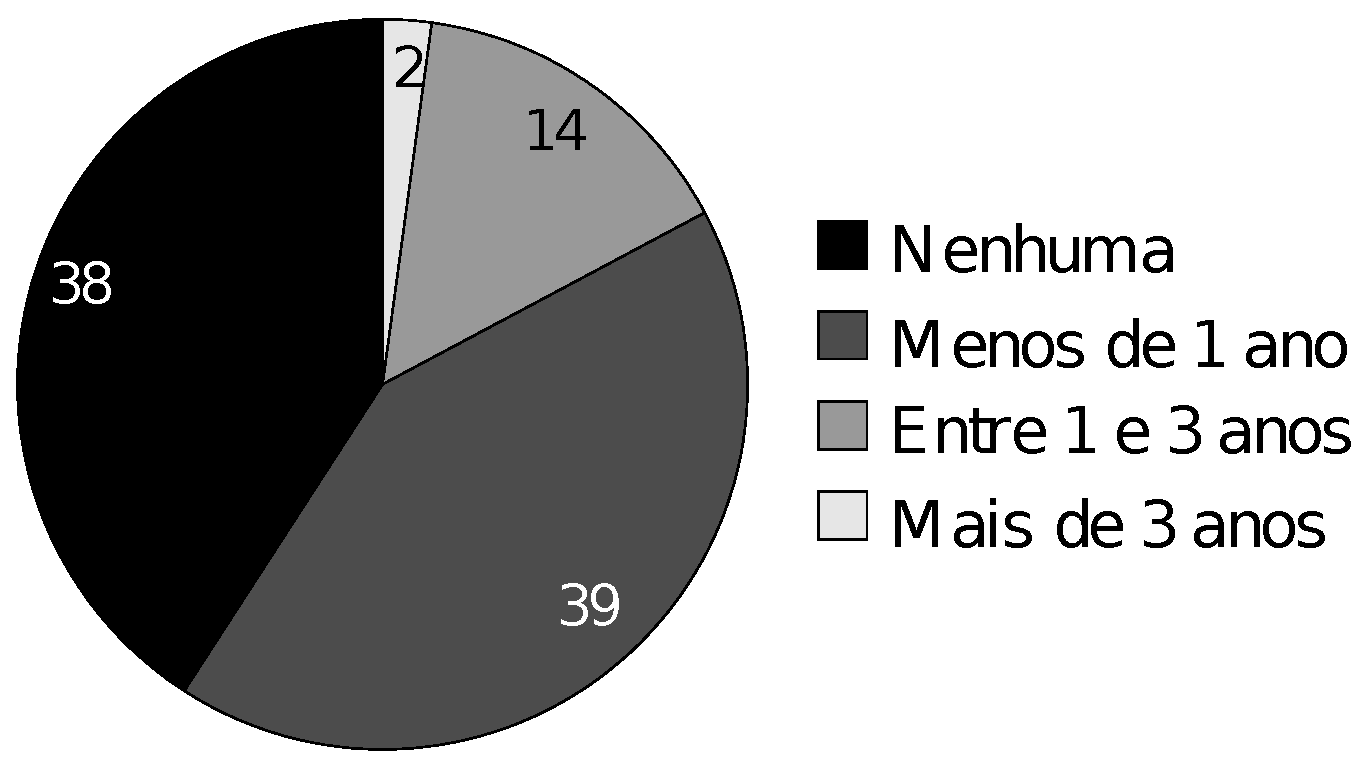
\includegraphics[scale=.3]{EA-experienciaMA}
    \caption{Experiência dos participantes com métodos ágeis}
    \label{fig:EA-experienciaMA}
  \end{minipage}
\end{figure}

A figura \ref{fig:EA-atividades} mostra a distribuição de atividades
dos participantes. A maioria dos participantes eram desenvolvedores e,
em segundo lugar, gerentes. A figura \ref{fig:EA-experienciaMA} mostra
que a grande maioria tinham pouca experiência com métodos
ágeis. Unindo esse dado com o fato de que 82\% tinham menos de 35 anos
de idade, os participantes podem ser caracterizados como uma população
de jovens profissionais com interesse em métodos ágeis mas com
conhecimento superficial sobre o assunto. Do ponto de vista do
software livre, 67\% das respostas diziam nunca ter contribuído com
software livre e 24\% afirmavam colaborarem ocasionalmente com algum
projeto.

Esses resultados mostram que a população interessada em métodos ágeis
tem pouco envolvimento com a comunidade de software livre. Vale também
notar que a correlação entre a experiência em métodos ágeis e as
contribuições com métodos ágeis na pesquisa era muito pequena para
afirmar qualquer coisa. Esse trabalho procura identificar melhor a
relação entre esses dois mundos identificando os pontos de proximidade
e distância assim como os potenciais elementos de melhora em cada
ambiente.

%% ------------------------------------------------------------------------- %%
\section{Contribuições}
\label{sec:contribucoes}

As principais contribuições deste trabalho estão discriminadas abaixo:

\begin{itemize}
\item Um estudo detalhado sobre as semelhanças e diferenças entre
  métodos ágeis e software livre;
\item Uma pesquisa relacionando métodos ágeis e software livre;
\item Uma pesquisa com a comunidade de software livre sobre sua
  relação com métodos ágeis;
\item Uma pesquisa com a comunidade de métodos ágeis sobre sua relação
  com software livre e
\item Uma análise de Programação Extrema \cite{XP01} sob o ponto de
  vista do \emph{Open Source Maturity Model} (OMM) do projeto
  QualiPSo.
\end{itemize}

%% ------------------------------------------------------------------------- %%
\section{Organização do Trabalho}
\label{sec:organizacao_trabalho}

Os tópicos apresentados nesse trabalho consideram apenas um
subconjunto de projetos que são ditos ágeis ou software livre. O
Capítulo \ref{cap:escopo} apresenta o escopo dos projetos abordados
nesse trabalho. O Capítulo \ref{cap:semelhancas} apresenta argumentos
que levam a crer que métodos ágeis estão fortemente ligados com
software livre e levaram à elaboração de dois questionários
apresentados no Capítulo \ref{cap:pesquisas}. Os questionários
procuraram identificar os maiores problemas percebidos em cada
comunidade e ferramentas que poderiam ajudar a minimizar esses
problemas. O capítulo ainda traz uma análise das respostas obtidas nos
questionários.  Em seguida, no Capítulo \ref{cap:diferencas}, são
destacadas as diferenças nos princípios diferentes na comunidade que
as respostas do questionário apresentaram. O Capítulo \ref{cap:omm}
analisa como um método ágil resolve as questões levantadas pelo Modelo
de Maturidade Aberto ({\it Open Maturity Model}) do projeto QualiPSo.
Por fim, o Capítulo \ref{cap:conclusoes} resume o trabalho realizado e
apresenta futuros trabalhos.
